\documentclass[12pt]{extarticle}
\usepackage{ucs}
\usepackage[utf8x]{inputenc}
\usepackage{amsmath}
\usepackage{amssymb}
\usepackage{tikz}
\usepackage[unicode, pdftex]{hyperref}
\usepackage[russian]{babel}
\usepackage[T2A]{fontenc}
\usepackage{pgfplots}
\usepackage{amsthm}
\usepackage{latexsym}
\usepackage{mathtools}
\usepackage{listings}
\usepackage{color}
\usepackage{graphicx}
\usepackage{float}
\usepackage{wrapfig}
\title{Лингвистические нейросети, проходящие тест Тьюринга}
\author{Ларин Глеб}

\newtheorem*{remark}{Замечание}
\newtheorem{lemma}{Лемма}
\newtheorem*{definition}{Определение}
\newtheorem*{example}{Пример}

\lstset{ 
  belowcaptionskip=1\baselineskip,
  breaklines=true,
  frame=L,
  xleftmargin=\parindent,
  language=C++,
  showstringspaces=false,
  basicstyle=\footnotesize\ttfamily,
  keywordstyle=\bfseries\color{green!40!black},
  commentstyle=\itshape\color{purple!40!black},
  identifierstyle=\color{blue},
  stringstyle=\color{red},
}
	
\begin{document}


\maketitle
	\centerline{\textbf{0. Вступление.}}
	В современном мире остро стоит проблема создания искуственного разума. Один из тестов, способных дать ответ на вопрос о разумности субъекта, является Тест Тьюринга. В данной работе мы попробуем реализовать нейросеть, способную обучиться русскому языку на уровне достаточном для прохождения данного теста.
	
	\centerline{\textbf{I. Программирование математической состовляющей.}}
	\centerline{\textbf{Производные.}}
	Человек, благодаря развитому абстрактному мышлению, может представить себе бесконечность (в данном случае бесконечно малые), а от сюда и множественные математические идеи, которые строятся на ей. Одна из них - это производная. \newline
	
	Рассмотрим классическое определение производной:
	
	\centerline{$f'(x) = \displaystyle\lim_{\Delta x\to0} \frac{f(x+\Delta x) - f(x)}{\Delta x} $} 
	
	Благодаря формализации предела, человек может его понять, а как следствие, понять и производную. \newline
	
	Машина же не понимает слово стремится, потому что ей необходимы точные вычисления. В данном случае прибегнем к численному дифференцированию. 
	
	Убирая понятие предела, мы получаем:
	
	\centerline{$f'(x) = \frac{f(x+h) - f(x)}{h} $} 
	
	Где $h \rightarrow 0$ - шаг аппроксимации. \newpage
	Формулу (1.1) называют \textit{правой разностью} и аналогичным образом можно вывести формулу \textit{левой разности}:
	
	\centerline{$f'(x) = \frac{f(x) - f(x-h)}{h}$} 
	
	Чтобы найти ошибку правой и левой разности, разложим следующие функции в ряд Тейлора в точке x:
	
	\centerline{$f(x+h) = \displaystyle \sum_{k=0}^{n} \frac{f^{(k)}(x)}{k!}*(x+h-x)^k=\displaystyle \sum_{k=0}^{n} \frac{f^{(k)}(x)}{k!}*(h)^k$ (1.1)} 
	\centerline{$f(x-h) = \displaystyle \sum_{k=0}^{n} \frac{f^{(k)}(x)}{k!}*(x-h-x)^k=\displaystyle \sum_{k=0}^{n} \frac{f^{(k)}(x)}{k!}*(-h)^k$ (1.2)}
	
	Учитывая, что нам нужна только первая производная, то $n=1$. 
	
	\centerline{$f(x+h) = \displaystyle \sum_{k=0}^{1} \frac{f^{(k)}(x)}{k!}*(h)^k = f(x) + hf'(x) + \frac{R_1(x+h)}{h}$}
 	\centerline{$f(x-h) = \displaystyle \sum_{k=0}^{1} \frac{f^{(k)}(x)}{k!}*(-h)^k = f(x) - hf'(x) + \frac{R_1(x-h)}{h}$}
	
	Тогда:
	
	\centerline{$f'(x) = \frac{f(x+h) - f(x)}{h} + \frac{R_1(x+h)}{h} $} 
	\centerline{$f'(x) = \frac{f(x+h) - f(x)}{h} + \frac{R_1(x+h)}{h} $}
	
	Запишем же остаточный член в форме Лагранжа:
	
	\centerline{$R_1(x \pm h) = \frac{(x \pm h - x) ^ {1+1}}{(1+1)!} f^{(1+1)}[x+ \theta(x \pm h - x)] = \frac{h ^2}{2!} f''(x \pm \theta* h)$}
	\centerline{$\theta \in (0,1)$}
	
	Минимализируя шаг аппроксимации, получаем:
	
	\centerline{$\displaystyle \lim_{h \rightarrow 0} \theta h = 0$}
	
	Значит остаточный член, используя нотацию О-большого:
	
	\centerline{$R_1(x \pm h) = \frac{h ^2}{2} f''(x) = O(h^2) (1.3)$}
	
	Тогда погрешность левой и правой разности:
	
	\centerline{$f'(x) = \frac{f(x+h) - f(x)}{h} + \frac{O(h^2)}{h} = \frac{f(x+h) - f(x)}{h} + O(h)$} 
	\centerline{$f'(x) = \frac{f(x+h) - f(x)}{h} + \frac{O(h^2)}{h} =\frac{f(x+h) - f(x)}{h} +O(h)  $}
	
	\newpage
	Формулу (1.4) называют \textit{центральной разностью}. Именно её мы и будем использовать:
	
	\centerline{$f'(x) = \frac{f(x+h) - f(x-h)}{2h}$ (1.4)} 
	
	Чтобы найти её ошибку, вычтем из (1.2) формулу (1.1):
	
	\centerline{$f(x+h) - f(x-h) = 2*\displaystyle \sum_{k=0}^{n} \frac{f^{(2k+1)}(x)}{(2k+1)!}h^{2k+1}$}
	
	Поскольку нам нужна только первая производная, то $n = 1$:
	
	\centerline{$f(x+h) - f(x-h) = 2*\displaystyle \sum_{k=0}^{1} \frac{f^{(2k+1)}(x)}{(2k+1)!}h^{2k+1} + R_1(x+h) = 2(hf'(x) + R_2(x+h))$}
	
	\centerline{$\frac{f(x+h) - f(x-h)}{2} = hf'(x) + R_2(x+h)$}
	
	Аналогично выводу (1.3), получаем: \newline
	\centerline{$R_2(x+h) = \frac{f'''(x)}{3!}h^3 = O(h^3)$}
	
	Подставляя в центральную разность:
	
	\centerline{$\frac{f(x+h) - f(x-h)}{2} = hf'(x) + O(h^3)$}
	\centerline{$\frac{f(x+h) - f(x-h)}{2h} -  \frac{O(h^3)}{h} = f'(x)$}
	\centerline{$\frac{f(x+h) - f(x-h)}{2h} + {O(h^2)} = f'(x)$ (1.5)}
	
	Как мы видим, здесь ошибка много лучше, чем при использовании правой или левой разности. Конечно, мы можем продолжать раскладывать в ряд $f(x+2h)$, получая формулы двойной, четверной и прочих разностей, но тут вступает в силу погрешность вычисления компьютера. 
	
	Действительно, пусть $\epsilon \approx 10^{-16}$ - максимальная точность, которую может дать С++ (double). Полагая, что $\epsilon(x)\leq\epsilon$ - ошибка, которая получается при вычислении в точке х, мы получаем:
		
	\centerline{$\tilde{f}(x) = f(x) + \epsilon(x)$}
	\centerline{$\tilde{f}'(x) = f'(x) + \epsilon'(x)$} 
	 
	 
	\begin{remark}
		В данном контексте мы не рассматриваем ошибку аппроксимации, которая получилась в формулах выше.
	\end{remark}
	\centerline{$|\epsilon'(x)| = |\frac{\epsilon(x+h) - \epsilon(x)}{h}| \leq \frac{2\epsilon}{h}$}
	
	Таким образом, нетрудно вычислить и оптимальное h с учётом использования центральной разности, где ошибка аппроксимации $O(h^2)$:
	
	\centerline{$|f'(x) - \tilde{f}'(x)| = O(h^2) + \frac{2\epsilon}{h} $}
	
	Исходя из (1.3):
	
	\centerline{$O(h^2) = \frac{h^2}{2}f''(x)$}
	\centerline{$|f'(x) - \tilde{f}'(x)| = \frac{h^2}{2}f''(x) + \frac{2\epsilon}{h} $}
	
	Минимум же получается, если $\frac{h^2}{2}f''(x) = \frac{2\epsilon}{h}$, откуда h:
	
	\centerline{$h \approx \sqrt[3]{\frac{4\epsilon}{f''(x)}}$}
	
	Значит наилучший порядок оценки получается при $\sqrt[3]{\epsilon}$.
	
	Аналогично для любой из разностей, но для расчёта полной ошибки двойной разности, например, потребуются производные высших порядков, что вызывает затруднение, в отличии от двойной производной.
	
	Реализация этого на С++:
	
	\begin{lstlisting}
float approximation__devirate(function* __function, float __point_devirative,  float __derivative_step = APPROXIMATION_ORDER) {
    return ((*__function)(__point_devirative + __derivative_step) - (*__function)(__point_devirative - __derivative_step))/(2 * __derivative_step);
}
	\end{lstlisting}
						
	\centerline{\textbf{Частные производные и градиент.}}
	Для работы нейросетей необходимо запрограммировать возможность вычисления частных производных. Нам помогут выкладки, которые мы получили выше. 
	
	Пусть нам дана функция $f(x_1, x_2 \dots x_n)$. Исходя из определения частой производной в точке $(a_1, a_2 \dots a_n)$:
	
	\centerline{$ \frac{\partial f}{\partial x_i}(a_1, a_2 \dots a_n) = \displaystyle\lim_{\Delta x \rightarrow 0}\frac{f(a1 \dots a_i + \Delta x_i \dots a_n) - f(a_1, a_2 \dots a_n) } {\Delta x} $}
	
	Аналогично формуле (1.5) можно получить центральную разность для частных производных:
	
	\centerline{$\frac{f(a1 \dots a_i + h_i \dots a_n) - f(a1 \dots a_i - h_i \dots a_n)}{2h_i} + O(h_i^2) = \frac{\partial f}{\partial x_i}(a_1, a_2 \dots a_n)$ (1.6)}  
	
	Где $h_i \rightarrow 0$ - шаг аппроксимации при нахождении производной по i-ому аргументу функции. Учитывая, что все остальные аргументы принимаются за константу, то вывод $O(h_i^2)$ остаётся преждним. 
	
	Пользуясь формулой (1.6) можно легко численно посчитать градиент. 
	
	Пусть $\omega$ - функция от n переменных. Если же мы хотим вычислить градиент в точке $(a_1, a_2 .. a_n)$, то будет верна следующая формула:
	
	\centerline{$\nabla \omega(a_1, a_2 .. a_n) = (D_1\omega(a_1, a_2 .. a_n), \dots D_n\omega(a_1, a_2 .. a_n))$}
	\centerline{$D_i \omega = \frac{\partial \omega}{\partial x_i}$}
	\newpage
	Ошибка же вычисления градиента будет сумма ошибок всех вычислений частных производных с помощью центральной разности:
		
		\centerline{$\Theta = \displaystyle\sum_{i=0}^{n} O(h_i^2)$}
	
	Или же, если нам нужен вектор ошибки:
	
		\centerline{$\Theta_v = (O(h_1^2), O(h_2^2)... O(h_n^2))$}
		
	Где $O(h_i^2)$ вычисляется аналогично формуле (1.3):
	
		\centerline{$O(h_i^2) = \frac{h_i^2}{2} \frac{\partial^2 \omega}{\partial h_i^2}(a_1, a_2... a_n)$}
		
	Тогда градиент с учётом ошибки:
	
		\centerline{$\nabla \omega(a_1, a_2 .. a_n) = (D_1\omega(a_1, a_2 .. a_n), \dots D_n\omega(a_1, a_2 .. a_n)) + \Theta_v$}
	
	Реализация этого на С++:
	
		[Будет в дальнейшем]
		
	\centerline{\textbf{Матрицы.}}
		
		Кажется тривиальным, что для использования матриц подойдут двухмерные массивы или массив массивов. Да, это верно, но давайте рассмотрим обращение к таким объектам с помощью адрессной арифметики (рисунок один, так как для них будет одинаковое обращение):
		
	\begin{figure}[h]
			\centering
			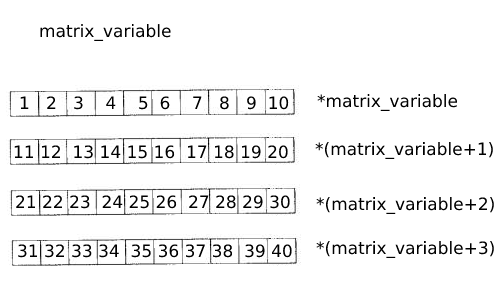
\includegraphics[width=0.8\linewidth]{matrix_1.png}
			\caption{Представление матрицы в виде двухмерного массива.}
			\label{fig:mpr}
	\end{figure}
	
	\newpage
	
	Чтобы получить какое-то $a_{ij}$, во-первых, необходимо получить его строку.
	
	Как мы видим, в памяти *\texttt{matrix\_variable} хранит массив, соответсвующий первой строке, *(\texttt{matrix\_variable}+1) - массив, соответсвующий второй строке и так далее.
	
	Чтобы получить уже элемент из нужного нам массива, опять обратимся к адресной арифметике:
	
	
	
	\begin{figure}[h]
			\centering
			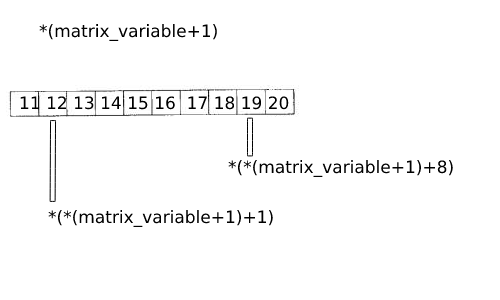
\includegraphics[width=0.8\linewidth]{matrix_2.png}
			\caption{Представление строки матрицы.}
			\label{fig:mpr}
	\end{figure}
	

	Получаем два указателя на один элемент. При работе с большими матрицами обращение через двойные указатели - это дорогая операция, а также зачастую неизвестно, куда ведёт такой двойной указатель: на следующую физическую ячейку, или на ячейку с каким-то случайным адресом - это остаётся проблемой. 
	Посчитаем количество тиков, которые занимает в таком случае обращение с помощью двойного указателя (рис 3).
	
	\begin{figure}[h]
			\centering
			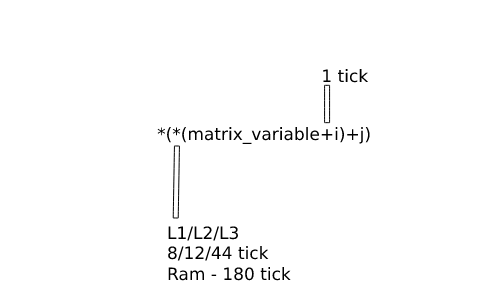
\includegraphics[width=0.8\linewidth]{matrix_3.png}
			\caption{Стоимость операций.}
			\label{fig:mpr}
	\end{figure}
	Исходя из \cite{litlink4} можно установить, что: 
	
	Стоимость сложения - 1 тик. 
	
	Стоимость обращения памяти зависит от того, куда попала наша переменная: в кэш, или в оперативную память, потому возьмём среднее значение - 61 тика.
	Суммарно вышло 124 тика.
	\newpage
	\begin{remark}
		На различных процессорах данные значения могут отличаться, потому мы взяли среднее значение. Также, у процессора есть несколько уровней кеширования, и на (рис 3) они обозначены L1, L2 и L3 соответственно.
	\end{remark} 
	
	Рассмотрим же другой способ представления матрицы: через одномерный массив. Исходя из (рис 4) легко понять работу такого метода: при объявлении матрицы он будет заполнять столбец, а после перейдёт на следующий. На (рис 4) массив будет представлен либо матрицой 2х5, либо 5х2.
	\begin{figure}[h]
			\centering
			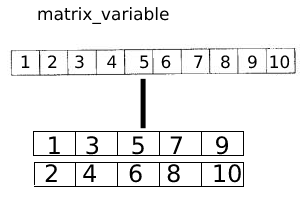
\includegraphics[width=0.4\linewidth]{matrix_4.png}
			\caption{Представление через одномерный массив.}
			\label{fig:mpr}
	\end{figure}
	
	\newpage
	
	\begin{remark}
		Фактически на линейном массиве мы организуем двойной.
	\end{remark}
	Теперь же разберёмся с обращением к такому массиву (рис 5).Чтобы получить какой-то элемент $a_{ij}$, мы будем применять формулу:
	
	\centerline{\texttt{*(matrix\_variable+N\_ROW*j+i)}}
	
	N\_ROW - количество строк в матрице. Может показаться, что таким образом мы будем хранить лишнее значение, которое добавит стоимость к операции обращения, но, во-первых, это значение нам заранее известно; во-вторых, в любом случае хранить размерность матриц необходимо для проверки при сложении и умножении, нахождении определителя.
	
	Посчитаем количество тиков в таком случае:
	
	Два сложения: 2 тика. 
	Одно умножение: 4 тика (среднее значение).
	Обращение к памяти: 61 тик. 
	
	Суммарно вышло 67 тиков, что быстрее более чем в полтора раза, чем двухмерный массив, потому вся дальнейшая реализация матриц будет строиться именно на одномерном массиве. 
		
	\begin{figure}[h]
			\centering
			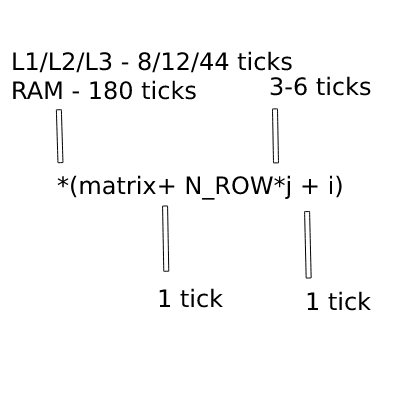
\includegraphics[width=0.4\linewidth]{matrix_5.png}
			\caption{Представление через одномерный массив.}
			\label{fig:mpr}
	\end{figure}
	
	
	\newpage
	
	
		\centerline{\textbf{II. Принцип работы нейросетей.}}
				\centerline{\textbf{Нейрон, активационная функция, индексация.}}
	Как и в мозге млекопитающих, за любое действие мозга отвечает нейрон, так и в любой нейросети за действие отвечает его имитация, которая принимает входные данные и выдаёт единственное значение, потому за каждый нейрон будет отвечать некоторая \textit{активационная} функция $\phi$.
	
	Учитывая её использование в дальнейших алгоритмах, то есть необходимое условие, чтобы $\phi$ нам подходила:

	\textit{1. Функция $\phi$ должна быть гладкой.} 
	
	\textit{2. Функция $\phi$ должна быть непрерывной.}
	
	\textit{3. $E(\phi) \in \mathbb{R} $}


	Теперь же необходимо понять, какие данные принимает функция активации нейрона.
	
	\begin{figure}[h]
			\centering
			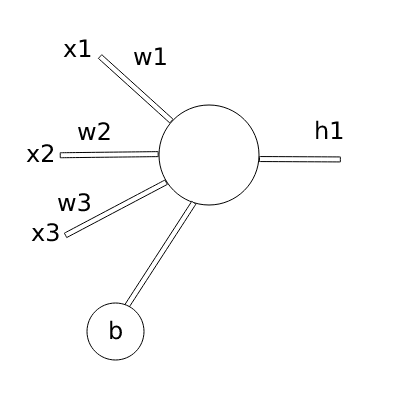
\includegraphics[width=0.4\linewidth]{neuron_1.png}
			\caption{Узел с несколькими входами.}
			\label{fig:mpr}
	\end{figure}
	
	
	На (рис 6) представлен узел. У каждого такого узла может быть больше входов, но каждый выход ведёт непросредственно в другой узел. Каждый вход и выход называется \textit{синапсом}. У каждого синапса есть некоторый коэффициент, называемый \textit{весом}. Система, состоящая из узла, синапса и активационной функции называется \textit{нейрон}.
	
	Вход же в активационную функцию рассчитывается следующей формулой:
	
	\centerline{$\displaystyle\sum_{i=0}^{n}x_iw_i + b $ (2.1)}
	
	В данном случае, n = 3 - количество входных синапсов, а b - коэффициент смещения. Он задерживает активацию нейрона (ниже будут представлены графики, где более подробно будет объяснено про роль коэффициента смещения).
	В таком случае выходной синапс нейрона:
	
	\centerline{$h_1 = \phi(\displaystyle\sum_{i=0}^{n}x_iw_i + b) $ (2.2)}
	В действительности современные нейросети содержат до нескольких миллардов нейронов \cite{litlink7}, из-за чего необходимо рассмотреть более сложную архитектуру:
	
	\begin{figure}[h]
			\centering
			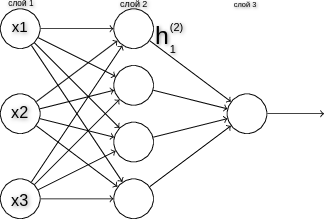
\includegraphics[width=0.7\linewidth]{neuron_2.png}
			\caption{Более комплексная система нейронов.}
			\label{fig:mpr}
	\end{figure}
	
	Слой, содержащий три нейрона (cлой 1), называется \textit{входным}, а содержащий один нейрон (слой 3) \textit{исходным}. Все слои, расположенные между этими двумя, называются \textit{скрытыми}.
	
	Так как каждые два нейрона содержат синапс, у каждого синапса свой вес, то необходимо ввести индексацию: $w_{ij}^{(l)}$
	
	i - номер узла в l+1 слое, а j - номер узла в l-ом слое (куда-откуда). Например $w_{21}^{(1)}$ означает вес синапса между вторый нейроном во втором слое и первым нейроном первого слоя.
	
	Аналогично для каждого нейрона есть коэффициент смещения, потому введём индексацию для него: $b_i^{(l)}$ - номер i-ого нейрона в l+1 слое.
	
	
	Выходное значение будем обозначать за $h_i^{(l)}$, где i - номер нейрона в l-ом слое.
	
	Выход исходного слоя обозначим $H$. 
	
	В таком случае перепишем (2.2) с учётом новой индексации:
	
	\centerline{$h_i^{(l)} = \displaystyle\phi(\underbrace{\sum_{k=0}^{n}w_{ik}^{(l-1)}x_k + b_i^{(l-1)}})$ (2.3)}
	\centerline{   $z_i^{(l)}$}
	
	Или же:
	
	\centerline{$h_i^{(l)} = \displaystyle\phi(z_i^{(l)})$ (2.3)}
		
	
	\centerline{\textbf{Процесс прямого распространения.}}
	
	\begin{remark}
		Все дальнейшие вычисления будут проводиться для системы нейронов, представленных на (рис 7), но они верны и для произвольной системы.
	\end{remark}
	
	Чтобы рассчитать H по заданным данным, мы воспользуемся формулой (2.3) и применим её для нашей системы на (рис 7):
	
	\centerline{$h_1^{(2)} = \phi(w_{11}^{(1)}x_1 + w_{12}^{(1)}x_2  + w_{13}^{(1)}x_3 + b_1^{(1)})$}
	\centerline{$h_2^{(2)} = \phi(w_{21}^{(1)}x_1 + w_{22}^{(1)}x_2  + w_{23}^{(1)}x_3 + b_2^{(1)})$}
	\centerline{$h_3^{(2)} = \phi(w_{31}^{(1)}x_1 + w_{32}^{(1)}x_2  + w_{33}^{(1)}x_3 + b_3^{(1)})$}
	\centerline{$H = h_1^{(3)} = \phi(w_{11}^{(2)}h_1^{(2)} + w_{12}^{(2)}h_2^{(2)}   + w_{13}^{(2)}h_3^{2} + b_1^{(2)})$}
	
	Для расчёта H вместо входных данных $x_i$ мы используем выходные данные от синапсов $h_i$. Аналогично будем делать, если в нашей системе несколько слоёв: выходный синапс одного нейрона является входным синапсом другого нейрона.
	
	Данная нотация прекрасно читается в случае малых размеров системы нейронов, но при большом их количестве, данная запись становится громодской, потому её можно записать через матрицы. Для этого мы введём следующее обозначение:
	
	\centerline{ $H^{(l)} = \begin{pmatrix}
		h_1^{(l)} \\
		\vdots \\
		h_n^{(l)}
	\end{pmatrix}$ (2.4)}
	
	В нашем случае же случае:
	
	\centerline{$H^{(2)} = \begin{pmatrix}
		h_1^{(2)} \\
		h_2^{(2)} \\
		h_3^{(2)}
	\end{pmatrix}$}
	
	Немного изменим $\phi$: теперь она будет принимать матрицу и возвращать матрицу:
	
	\centerline{$H^{(2)} = \begin{pmatrix}
		h_1^{(2)} \\
		h_2^{(2)} \\
		h_3^{(2)}
	\end{pmatrix} = \phi\begin{pmatrix}
		w_{11}^{(1)}x_1 + w_{12}^{(1)}x_2  + w_{13}^{(1)}x_3 + b_1^{(1)} \\
		w_{21}^{(1)}x_1 + w_{22}^{(1)}x_2  + w_{23}^{(1)}x_3 + b_2^{(1)} \\
		w_{31}^{(1)}x_1 + w_{32}^{(1)}x_2  + w_{33}^{(1)}x_3 + b_3^{(1)} \end{pmatrix}$}
	Поподробнее рассмотрим матрицу, которая является агрументом:
	
	\centerline{$\begin{pmatrix}
		w_{11}^{(1)}x_1 + w_{12}^{(1)}x_2  + w_{13}^{(1)}x_3 + b_1^{(1)} \\
		w_{21}^{(1)}x_1 + w_{22}^{(1)}x_2  + w_{23}^{(1)}x_3 + b_2^{(1)} \\
		w_{31}^{(1)}x_1 + w_{32}^{(1)}x_2  + w_{33}^{(1)}x_3 + b_3^{(1)} \end{pmatrix} = \begin{pmatrix}
		w_{11}^{(1)}x_1 + w_{12}^{(1)}x_2  + w_{13}^{(1)}x_3  \\
		w_{21}^{(1)}x_1 + w_{22}^{(1)}x_2  + w_{23}^{(1)}x_3  \\
		w_{31}^{(1)}x_1 + w_{32}^{(1)}x_2  + w_{33}^{(1)}x_3 \end{pmatrix} +\begin{pmatrix}
		b_1^{(1)} \\
		b_2^{(1)} \\
		b_3^{(1)} \end{pmatrix} $}
	
	\centerline{$\begin{pmatrix}
		w_{11}^{(1)}x_1 + w_{12}^{(1)}x_2  + w_{13}^{(1)}x_3  \\
		w_{21}^{(1)}x_1 + w_{22}^{(1)}x_2  + w_{23}^{(1)}x_3  \\
		w_{31}^{(1)}x_1 + w_{32}^{(1)}x_2  + w_{33}^{(1)}x_3 \end{pmatrix} +\begin{pmatrix}
		b_1^{(1)} \\
		b_2^{(1)} \\
		b_3^{(1)} \end{pmatrix} = \begin{pmatrix}
		w_{11}^{(1)} & w_{12}^{(1)} & w_{13}^{(1)}  \\
		w_{21}^{(1)} & w_{22}^{(1)} & w_{23}^{(1)}  \\
		w_{31}^{(1)} & w_{32}^{(1)} & w_{33}^{(1)} \end{pmatrix} * \begin{pmatrix}
		x_1  \\
		x_2\\
		x_3 \end{pmatrix} +\begin{pmatrix}
		b_1^{(1)} \\
		b_2^{(1)} \\
		b_3^{(1)} \end{pmatrix} $}
		
		Как мы видим, наша матрица является композицией нескольких: матрицы весов, входных синапсов и коэффициентов смещения. 
		
		
		Положим следующее:
		
		\centerline{$B^{(l)} = \begin{pmatrix}
		b_1^{(l)} \\
		\vdots \\
		b_n^{(l)} \end{pmatrix} $}
		
		\centerline{$W^{(l)} = \begin{pmatrix}
		w_{11}^{(l)} & \cdots & w_{1i}^{(l)} \\ 
		\vdots & \ddots & \vdots \\
		w_{j1}^{(l)} & \dots & w_{ji}^{(l)} \end{pmatrix}$}
		
	Тогда наш выходной слой в новых обозначениях:
	
	
	\centerline{$H^{(2)} =\phi(W^{(1)} * H^{(1)} +  B^{(1)})$}
	
	\begin{remark}
		$H^{(1)}$ - матрица входных значений нейросети.
	\end{remark}
	
	Исходя из этого:
	
	\centerline{$H = H^{(3)} = \phi(W^{(2)} *H^{(2)} +  B^{(2)})$}
	
	В дальнейшем будет пользоваться этим в общем виде:
	
	\centerline{$H^{(l)} =  \phi(W^{(l-1)} * H^{(l-1)}+ B^{(l-1)})$}
	
	
	\centerline{\textbf{Процесс обратного распространения. Градиентный спуск. }}
	
	Весь процесс обучения нейросети заключается в верной корректировке значений всех весов нейросети. Фактически, вся нейросеть - это большая функция, принимающая тысячи значений весов и сдвигов. 
	
	Наиболее вероятным способом обучения нейросети является пара "вход-выход". Рассмотрим пример:
	
	
	\centerline{$X = \begin{pmatrix}
	abstract input 1 \\
	abstract input 2\\
	abstract input 3\\
	\vdots
	\end{pmatrix}$}
	
	\centerline{$Y = \begin{pmatrix}
	abstract output 1 \\
	abstract output 2\\
	abstract output 3\\
	\vdots
	\end{pmatrix}$}
	
	Каждому $X_i$ соответсвует одно $Y_i$. X - матрица всех входов, которые принимает нейросеть, а Y - матрица её выхода. Эти значения мы заранее знаем: например, обучая нейросеть опознавать картинки, мы знаем что на ней изображено. 
	
	\begin{remark}
		Все входные и выходные данные будут обработаны, став числовыми значениями, поскольку сама нейросеть работает с числами, потому в дальнейшем мы будем использовать именно их.
	\end{remark}
	
	Но как скорректировать веса, зная $X_i$ и $Y_i$? Очевидно, что нейросеть в любом случае даст какой-либо выход - $O = H^{(L)}$, где $L$ - количество слоёв в нейросети. В тоже время мы знаем, что у нас есть заранее четкие значения для данных входных параметров (пример: мы заранее знаем, что за цифра на картинке). Тогда возьмём некоторую функцию $\lambda(O, E)$, которая будет рассчитывать отклонение от ожидаемых значений. В дальнейшем это будет \textit{функцией ошибки}. 
	
	Чтобы понять, а как нам корректировать весы, мы рассмотрим простой пример. Пусть наша нейрость схожа с нейросетью на  рис. 8:
		
	\begin{figure}[h]
			\centering
			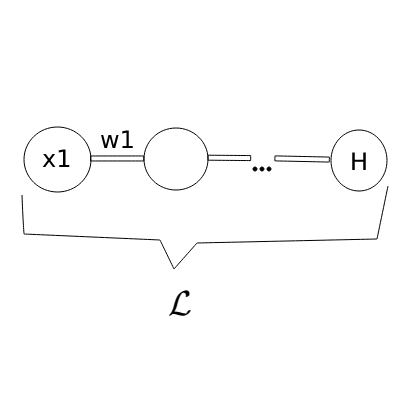
\includegraphics[width=0.5\linewidth]{neuron_algorithm.png}
			\caption{Нейросеть с функцией ошибки $\mathcal{L}$.}
			\label{fig:mpr}
	\end{figure}
	
	\newpage
	
	Тогда функция ошибки будет: 
	
			\centerline{$\mathcal{L}(w^{(1)}, b^{(2)}, \dots w^{(L)}, b^{(L)})$ или}
			\centerline{$\mathcal{L}(\{w^{(i)}\}, \{b^{(i)}\})$}
	
	 В тоже время функция ошибки - это функция оценки: ошибка и является отклонением от ожидаемых значений. Запишем это в следующем виде:
	
	\centerline{$\mathcal{L}(\{w^{(i)}\}, \{b^{(i)}\}) = \lambda(O, E)$}
	Поскольку в данном примере у каждого нейрона всего два синапса(входной и выходной), то индексацию можно опустить в силу её очевидности.
	Мы формализовали нашу проблему: заместо какой-то случайной корректировки весов, мы будем искать такие $\{w^{(j)}\}$ и $\{b^{(j)}\}$, что при таких значениях достигается $\min(\mathcal{L})$. Для этого мы будем использовать \textit{градиентный спуск}.
	
	Учитывая, что нам известен конечный выход (Y), то мы будем идти с конца. Пусть ошибка при заданных выходных данных - это $\mathcal{L}_0$.
	Рассмотрим, как зависит $\mathcal{L}_0$ от $w^{(L)}$:
	
	\centerline{$\frac{\partial \mathcal{L}_0}{\partial w^{(L)}}$}
	
	Но мы знаем, что $\mathcal{L}_0$ зависит в любом случае от $z^{(L)}$, которое зависит от $w^{(L)}$. Тогда по цепному правилу:
	
	\centerline{$\frac{\partial \mathcal{L}_0}{\partial w^{(L)}} = \frac{\partial z^{(L)}}{\partial w^{(L)}}\frac{\partial h^{(L)}}{\partial z^{(L)}}\frac{\partial \mathcal{L}_0 }{\partial h^{(L)}}$}
	
	Рассмотрим каждую частную производную по отдельности:
	
	\centerline{$\frac{\partial h^{(L)}}{\partial z^{(L)}} = \frac{\partial \phi}{\partial z^{(L)}} = \phi'(z^{(L)})$}
	
	\centerline{$\frac{\partial z^{(L)}}{\partial w^{(L)}} = \frac{\partial (w^{(L)}h^{(L-1)}+b^{(L)})}{\partial w^{(L)}} = h^{(L-1)}$}
	
	Но в тоже время, $h^{(L)}$ - это некоторое $o \in O$. Перепишем нашу частную производную в силу равенства функций:
	
	\centerline{$\frac{\partial \mathcal{L}_0 }{\partial h^{(L)}} = \frac{\partial \lambda}{\partial o}$}
	
	\centerline{$\frac{\partial \mathcal{L}_0}{\partial w^{(L)}} = h^{(L-1)}\phi'(z^{(L)})\frac{\partial \lambda}{\partial o}$}
	
	Аналогично несложно рассчитать для сдвига $b^{(l)}$:
	
	\centerline{$\frac{\partial \mathcal{L}_0}{\partial b^{(L)}} = \frac{\partial z^{(L)}}{\partial b^{(L)}}\frac{\partial h^{(L)}}{\partial z^{(L)}}\frac{\partial \mathcal{L}_0 }{\partial h^{(L)}}$}
	
	\centerline{$\frac{\partial h^{(L)}}{\partial z^{(L)}} = \frac{\partial \phi}{\partial z^{(L)}} = \phi'(z^{(L)})$}
	
	\centerline{$\frac{\partial z^{(L)}}{\partial b^{(L)}}= \frac{\partial(w^{(L)}h^{(L)}+b^{(L)})}{\partial b^{(L)}} = 1 \Rightarrow$}

	\centerline{$\Rightarrow \frac{\partial \mathcal{L}_0}{\partial b^{(L)}} = \phi'(z^{(L)})\frac{\partial \lambda}{\partial o}$}
	
	Сама же зависимость общей ошибки вычисляется, как среднее всех ошибок при всех данных (наборах):	

    \centerline{$\frac{\partial \mathcal{L}}{\partial w^{(L)}} = \overline{\frac{\partial  \mathcal{L}_k}{\partial w^{(L)}}}$}
	
	И это один из компонентов. Аналогично мы вычисляем зависимость от остальных сдвигов и весов (заменив $w^{(L)}$ на $b^{(L)}$, мы получаем  формулу для сдвига).
	
	Что делать, если у нас несколько синапсов, более комплексная архитектура, как на рисунке 7?
	
	Все будет аналогично, потому сразу запишем в общем виде:
	
	\centerline{$\frac{\partial \mathcal{L}_0}{\partial w_{ij}^{(l)}} = \frac{\partial \mathcal{L}_0}{\partial  h_i^{(l)}}\frac{\partial h_i^{(L)}}{\partial z_i^{(l)}}\frac{\partial z_i^{(l)}}{\partial w_{ij}^{(l)}}$}
	
	\centerline{$\frac{\partial h_i^{(l)}}{\partial z_i^{(l)}} = \phi'(z_i^{(l)})$}
	
	\centerline{$\frac{\partial z_i^{(l)}}{\partial w_{ij}^{(l)}} = h_j^{(l-1)}$}
	
	\centerline{$\frac{\partial \mathcal{L}_0}{\partial w_{ij}^{(l)}} = h_j^{(l-1)} \phi'(z_i^{(l)}) \frac{\partial \mathcal{L}_0}{\partial  h_i^{(l)}}$}
	
	Чтобы посчитать зависимость $\frac{\partial \mathcal{L}_0}{\partial  h_i^{(l)}}$, рассмотрим такую же в предыдущем слое:
	
	\centerline{$\frac{\partial \mathcal{L}_0}{\partial  h_i^{(l-1)}}$}
	
	Аналогично предыдущим выкладкам мы получаем частную производную, но теперь нам необходимо посчитать общую зависимость синапсов, потому просуммируем:
	
	\centerline{$\frac{\partial \mathcal{L}_0}{\partial  h_i^{(l-1)}} = \displaystyle \sum_{j = 1}^{n_l}\frac{\partial z_j^{(l)}}{\partial h_i^{(l-1)}}\frac{\partial h_j^{(l)}}{\partial z_j^{(l)}}\frac{\partial \mathcal{L}_0}{\partial  h_j^{(l)}} $}
	
	
	Исходя из выкладок выше, получаем:
	
	\centerline{$\frac{\partial \mathcal{L}_0}{\partial w_{ij}^{(l)}} = h_j^{(l-1)} \phi'(z_i^{(l)}) \displaystyle \sum_{r=1}^{n_l}w_{rj}^{(l+1)}\phi '(z_r^{(l+1)})\frac{\partial \mathcal{L}_0}{\partial h_r^{(l+1)}}$}
	Где $n_l$ - количество синапсов в l слое. Мы вывели все нужные нам формулы, но остаётся вопрос: "Как посчитать $\frac{\partial \mathcal{L}_0}{\partial h_r^{(l+1)}}$?". 
	
	Тут стоить вспомнить, что $\frac{\partial \mathcal{L}_0}{\partial h_i^{(L)}} = \frac{\partial \lambda}{\partial o_i}$. Отсюда и начнёт действовать наш алгоритм (отсюда же и название \textit{обратное распространение}). Резюмируя всё сказанное выше:
	
	
	
	Для любых $w_{ij}^{(L)}$:
	
	\centerline{$\frac{\partial \mathcal{L}_0}{\partial w_{ij}^{(L)}} = h_j^{(L-1)} \phi'(z_i^{(L)}) \frac{\partial \lambda}{\partial o_i}$}
	
	Для оставшихся $w_{ij}^{(l)}$:
	
	\centerline{$\frac{\partial \mathcal{L}_0}{\partial w_{ij}^{(l)}} = h_j^{(l-1)} \phi'(z_i^{(l)}) \displaystyle \sum_{r=1}^{n_l}w_{rj}^{(l+1)}\phi '(z_r^{(l+1)})\frac{\partial \mathcal{L}_0}{\partial h_r^{(l+1)}}$}
	
	Вся суть алгоритма в том, что отношение $\frac{\partial \mathcal{L}_0}{\partial h_r^{(l+1)}}$ мы посчитали на более высоком слое, потому эта величина нам известа.
	
	
	Также используем то, что ошибка является средним всех ошибок:
	
	\centerline{$\frac{\partial \mathcal{L}}{\partial w_{ij}^{(l)}} = \overline{\frac{\partial \mathcal{L}_k}{\partial w_{ij}^{(l)}}}$}
	
	Тогда для рассчёта минимума функции градиент будет равен:
	
	\centerline{$\nabla \mathcal{L} = \Big(\frac{\partial \mathcal{L}}{\partial w_{11}^{(1)}}, \dots, \frac{\partial \mathcal{L}}{\partial w_{ij}^{(L)}}, \frac{\partial \mathcal{L}}{\partial b_{1}^{(1)}}, \dots, \frac{\partial \mathcal{L}}{\partial b_{i}^{(L)}}\Big)$}
	Поскольку градиент функции показывает в каком направлении функция растёт, то взяв его со знаком минус, мы получим её убывание.
	
	\centerline{\textbf{Обучение нейросети с помощью градиентного спуска.}}
	\centerline{\textbf{Стохаический градиентный спуск.}}
	
	Чтобы разобраться в процессе нахождение подходящих весов, необходимо формализовать часть понятий. 
	
	\textit{Набором} называют пару (X, Y). Различают два вида наборов: \textit{учебный}, \textit{тестовый}. \textit{Датасетом} называется совокупность учебного и тестового набора. \textit{Поколением} называют полную итерацию всех учебных наборов и рассчётом ошибки для них. Тестовый же набор необходим для изучения точности работы нейросети. 
	
	Алгоритм (1) обучения с помощью градиетного спуска таков:
	
	1. Установить случайные $w$ и $b$.
	
	2.1 С помощью процесса прямого распространения рассчитать выход нейросети.
	
	2.2 С помощью процесса обратного распостранения рассчитать ошибку для данного учебного набора. 
	
	3. Повторять 2.1-2.2 пока не закончаться учебные наборы. 
	
	4. Рассчитать среднюю ошибку, исходя из значений, полученных в 2.2.
	
	5. Пусть $P$ - матрица всех весов и смещений. Они расположены также, как и аргументы $\mathcal{L}$. Тогда новые веса и смещения необходимо посчитать по формуле:
	
	\centerline{$P_n = P - \eta \nabla \mathcal{L}$}	
	
	Где $\eta$ - шаг обучения. Его необоходимо менять из поколения в поколения, чтобы попасть в минимум функции ошибки. 
	
	Возникает следующая проблема: учебных наборов может быть несколько десятков тысяч.
	
	\begin{remark}
		Учебных наборов для нейросетей, выполняющих простую работу: распозновать цифры, объекты, простой анализ данных. Например, у MNIST для распознования цифр на это выделено 60000 учебных и 100000 тестовых наборов. Для нейросетей, о которых речь пойдёт в дальнейшем, количество учебных наборов крайне велико: если один диалог или один документ считать ровно одним набором, то у LaMDA училась на 2.97 миллиардах и 1.12 миллиардах учебных наборах соотвественно, проанализируя более 1.56 триллионов слов - \cite{litlink5}
	\end{remark} 
	
	Алгоритм (1) необходимо будет выполнить для каждого учебного набора несколько раз, что невероятно долго, потому мы немного изменим его. 
	
	Учебные наборы мы разобьём на кластеры. Тогда зависимость ошибки будет вычисляться следующим образом:
	
	\centerline{$\frac{\partial \mathcal{L}_p}{\partial w^{(L)}} = \overline{\frac{\partial  \mathcal{L}_k}{\partial w^{(L)}}}$}
	
	Для соответствующего p-ого кластера мы посчитаем градиент:
	
	\centerline{$\nabla \mathcal{L}_p = \Big(\frac{\partial \mathcal{L}_p}{\partial w_{11}^{(1)}}, \dots, \frac{\partial \mathcal{L}_p}{\partial w_{ij}^{(L)}}, \frac{\partial \mathcal{L}_p}{\partial b_{1}^{(1)}}, \dots, \frac{\partial \mathcal{L}_p}{\partial b_{i}^{(L)}}\Big)$}
	
	И выполним алгоритм (1) не для всех учебных наборов, а для p-ого кластера. Затем мы перейдём к кластеру p+1 и т.д. Таким образом мы реализовали \textit{стохаический градиентный спуск}. Его суть в рассчёте градиента не для всех учебных наборов, а для кластера. Следующий же градиент уже будет рассчитываться с учётом новых весов и сдвигов, полученных в предыдущем наборе. 
	
	\newpage
	
	\centerline{\textbf{III. Преобразование входных данных.}}
	\centerline{\textbf{Препроцессинг.}}
	Всё это время мы говорили о входных данных как о числах, забывая о некотором препроцессинге, который переведёт эти данные в числовые значения. Очевидно, что перед конвертацией текстовых данных в числовые необходимо провести некоторые преобразования:
	
	1. Перевести все символы в нижний регистр. 
	
	2. Преобразовать все числа в числительные. 
	
	3. Удаление регулярных выражений. 
	
	После этого кажется тривиальным следующее решение: каждый символ, включая пробелы и знаки препинания в строке, превратить в число с помощью ASCII таблицы. 
	
	\begin{figure}[h]
			\centering
			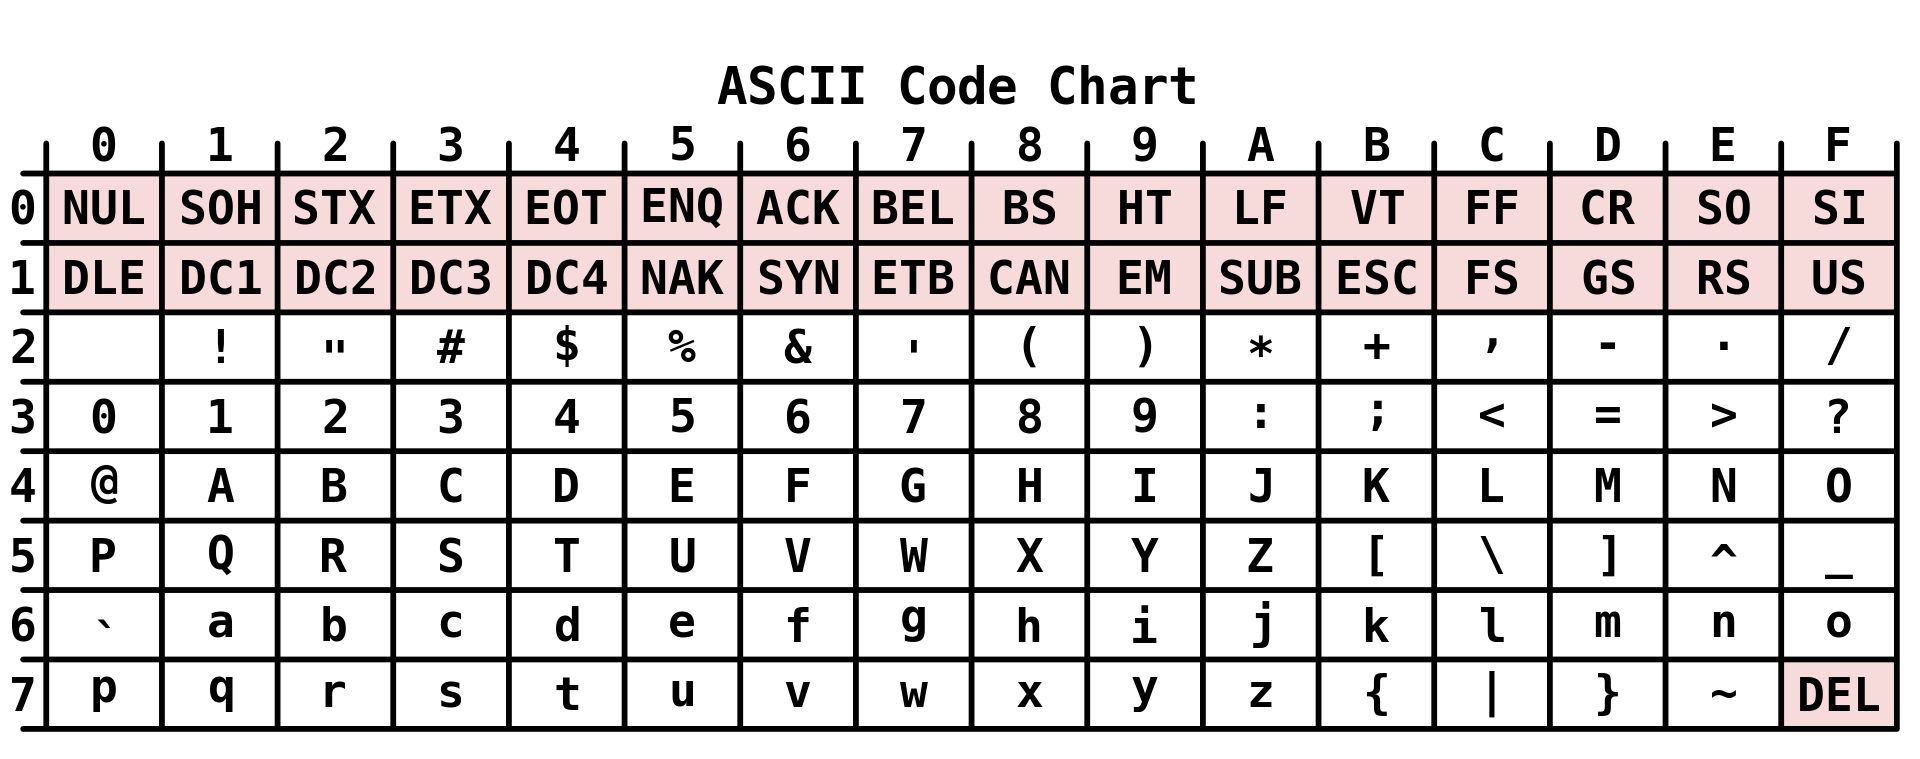
\includegraphics[width=0.8\linewidth]{ASCII_Code_Chart.png}
			\caption{Таблица ASCII.}
			\label{fig:mpr}
	\end{figure}
	
	Но в таком случае мы не учитываем очень важную вещь, которая и отличает последовательность случайных символов от языка: связь между словами, частями предложения, между самими предложениями. 
	
	Откажемся от этой идеи и будем анализировать части текста: предложения и слова. Рассмотрим ещё пару дополнительных этапов препроцессинга:

	1) Процесс формирования частей для анализа мы будем называть \textit{токенизация} или \textit{cегментация}. Токенизация бывает двух видов (как правило, эти виды последовательные, то есть в предпроцессинге идут поочерёдно): текст на предложения и предложение на токены. 
	
	Сегментация текста на предложения достаточно простой процесс: предложения отделены каким-то знаком пунктуации (точками в русском), потому разделить их несложно. Небольшая проблема заключается в опознании сокращений от конца предложения; для её решения используется словарь сокращений. 
	
	Сегментация предложения на токены (слова-компоненты) более тонкий процесс: слова разделены пробелами, а в некоторых языках, например, составные существительные пишутся через пробел; тем не менее, таких слов немного, потому определить такие слова исключения несложно. 
	
	 
	После образования токенов необходимо убрать ненужные части слов, которые не влияют на анализ текста. 
	
	\begin{example}
	"Я бежал по красной дороге"\ можно превратить в "Я бежать по красной дорога"\ - как мы видим, смысл предложения не теряется без падежей. Аналогично можно сказать "Я бег по красн дорог"\ - мы оставили только корни.
	\end{example} 
	
	2) Процессы, рассмотренные в примере, называются \textit{стемминг и лемматизация}.
	 	
	\textit{Стемминг} - процесс отрезания от слова "частей"\: приставок, суффиксов и пр. - в поиске основы слова. Правила для стеммера создаются заранее, что усложняет добавление новых языков; также "выкидывая" части слов можно потерять их смысл.
	
	\begin{example}
		Сравните: безветренный и основу -ветр-; ненужный и основу -нунж-; горевать и основу -гор-. 
	\end{example} 
	
	Конечно, стемминг позволяет привести слово к его основной форме, но часто можно потерять изначальное значение слово, что приведёт к некорректной обработке данных. 
	
	\textit{Лемматизация} же является альтернативой стемминга. Заместо "отрезания"\ частей для определения основы слов мы преобразуем форму слова в начальную: существительное в им. падеж, ед. число; глагол в инфинитив и пр.
	
	Отличие в том, что стеммер действует без знания контекста и, соответственно, не понимает разницу между словами, которые имеют разный смысл в зависимости от части речи.
	
	3) После обработки форм слов нам необходимо убрать все \textit{cтоп-слова}, которые не влияют на контекст: союзы, предлоги и т.д. Мы сами создаём данный стоп-словарь. 
	
	После препроцессинга у нас имеется набор токенов, который нам необходимо преобразовать в числовые данные. 
	
	\centerline{\textbf{Мешок слов. N-граммы. 
	Преобразование в числовые данные.}}
	
	Для конвертации числовой тип данных в текст нам необходимо понять, а какие именно слова мы использовали. Такой список мы будем называть \textit{словарём}, то есть некоторым множеством $D$, а i-ое предложение будет $S_i$ - множество слов после препроцессинга. 
	
	Чтобы превратить некоторое слово $\omega$ (дабы не путать с весами) в числовой тип данных мы будем вызывать некоторую функцию $C(\omega, i)$, которая вернёт нам число, исходя из слова. 
	
	
	Пусть множество слов на входе - $I$. \textit{Мешком/Вектором слов} называется множество следующего вида:
	
	\centerline{$B = \{ C(\omega_j, i) | \omega_j \in I \land \exists p: \omega_j \in D_p \} $}
	
	То есть множество, содержащее все возможные $C$. 
	
	Сложность этого метода в том, как определить словарь и как подсчитать вхождение слов: если у нас их большое количество, большой словарь, а сами входные данные неособо велики, то возникает множество ненужных нулей. 
	
	Чтобы решить это мы можем уменьшить размер словаря, формируя его не из отдельных слов, а из словосочетаний, например, или из трио слов. Данные совокупности называются \textit{N-граммами}, где N - количество слов. 
	
	Тогда наше $D^2_i$ будем представлять собой следующее: 
	
	\centerline{$D^2_i = \{\{S_j, S_{j+1} \} | S_j, S_{j+1} \in D_i \}$}  
	
	$D^2_i$ будет называться биграммой.
	
	В общем случае:
	
	\centerline{$D^n_i = \{\{S_j, S_{j+1} \dots S_{j+n} \} | S_j, S_{j+1} \dots S_{j+n} \in D_i\}$}  
	
	То есть набор n последовательных слов, содеращихся в \textit{первичном словаре} D. 
	
	Определим же базовый пример функции $C$:
	
	\[
    C(\omega, i)= 
	\begin{dcases}
    	1,& \text{if } \omega \in D_i \\
    	0,              & \text{otherwise}
	\end{dcases}
	\]
	
	Данная функция вернёт 1, если слово встречается в текущем предложении. Данный подход называется \textit{бинарным}, и он основан на логике: если мы говорим о некоторой теме, то и слова, которые нужны будут для неё, будут встречатся.
	
	Но бинарный подход плох отсутствием тонкой настройки. Если же попытаться создать функцию $C$ на основе частотности слова, то будет некорректная оценка слов. Один из способов исправить ситуацию - понижать оценку слова, которое часто встречается во всех схожих документах. Данный метод называется \textit{TF-IDF}. 
	Чтобы данный метод работал, мы введём некоторое множество всех входных текстов $\mathbf{I}$. Тогда можно рассмотреть две следующие функции:
	
	\centerline{$tf(\omega) = \frac{|D| - |D|\symbol{92}\{\omega\}}{|D|}$}
	
	\centerline{$idf(\omega, \mathbf{I}) = \log(\frac{|\mathbf{I}|}{
	\{\omega_i \in I | I \in \mathbf{I} \}|})$}
	
	\begin{remark}
	Фактически, $|D| - |D|\symbol{92}\{\omega\}$ - количество $\omega$ в множестве $D$, а $\{\omega_i \in I | I \in \mathbf{I} \}$ - число текстов из $\mathbf{I}$, где есть $\omega$.
	\end{remark}
	
	Тогда наши функции $C$ и множество $B$ можно переопределить как: 
	
	\centerline{$C(\omega, \mathbf{I}) = tf(\omega) * idf(\omega, \mathbf{I})$}
	
	\centerline{$B(I) = \{C(\omega_j, \mathbf{I}) | \omega_j \in I \land \exists p: \omega_j \in D_p \} $}
	
	На вход нейросети мы будем подавать B(I).
	
	\newpage	
\addcontentsline{toc}{section}{Список используемой литературы}
 
\begin{thebibliography}{}
    \bibitem{litlink1} В. А. Зорич, "Математический анализ .Часть I, II, III"\ , 10-ое издание

    \bibitem{litlink2}  Н.С.Бахвалов, Н.П.Жидков, Г.М.Кобельков,
"Численные методы"\ , учебное пособие

    \bibitem{litlink3} Р.З. Даутов, М.М. Карчевский, "Основы численных методов линейной алгебры"\ , учебное пособие
    
    \bibitem{litlink4} Agner Fog, “Instruction tables. Lists of instruction latencies, throughputs and micro-operation breakdowns for Intel, AMD and VIA CPUs”\ , стр 296-312 \newline
    
    \bibitem{litlink5} Romal Thoppilan, Daniel De Freitas, Jamie Hall Noam Shazeer and other,   "LaMDA: Language Models for Dialog Applications"\ , section 3
    
    \bibitem{litlink6} Loc Vu-Quoc, Alexander Hume, "Deep learning applied to computational mechanics: A comprehensive review, state of the art, and the classics"
    \bibitem{litlink7} Andrew Trask, David Gilmore, Matthew Russell, "Modeling Order in Neural Word Embeddings at Scale"\ - стр 8
    
    \bibitem{litlink8} Helmut Schmid, "Improvements In Part-of-Speech Tagging With an Application TO German "\
    
    \bibitem{litlink9} Helmut Schmid, "Probabilistic Part-of-Speech Tagging Using Decision Trees "\
    
    \bibitem{litlink10}Ilya Segalovich, " A fast morphological algorithm with unknown word guessing induced by a dictionary for a web search engine "\

\end{thebibliography}
\end{document}

